\chapter{Background}
\label{background}

We begin with different roles in the design, implementation and attack of a \ac{CPS}. We use the different categories to explain the attack model in Chapter 3 clearly. 
We provide a summary of \ac{CPS} after which we introduce conventional controller designs and their limitations. 
We further define \ac{DNN} based models and describe the open problems that exist in them. 
We then introduce the  general structure for \ac{MILP} modeling which we will later use in Chapter 5. 
We end with the formal description of our problem statement.

\section{Roles description}
There are three roles involved in designing and attacking \ac{CPS}. These are important to understand the different pieces of information an attacker needs to gather for attacking a system.

\begin{enumerate}
	\item \textbf{Specification Designer/Domain Expert:} The domain expert is responsible for designing the specification documents. 
	For an \ac{APS} the domain expert specifies the safe thresholds for the amount of insulin injected in a patient. The domain expert also indicates values that should trigger alarms, e.g., in case of a high blood glucose reading in \ac{APS}.
	\item \textbf{System Developer:} These are the people or the designers who
	build the \ac{DNN} architectures, e.g., an architect can use different types of \ac{ML} models such as decision trees, or \ac{DNN} to implement the system.
	\item \textbf{Attacker:} The attacker is trying to make the system misbehave by attacking the implementation of the \ac{CPS} without triggering safety alarms specified by the domain expert . 
\end{enumerate}

\begin{figure}
	\centering
	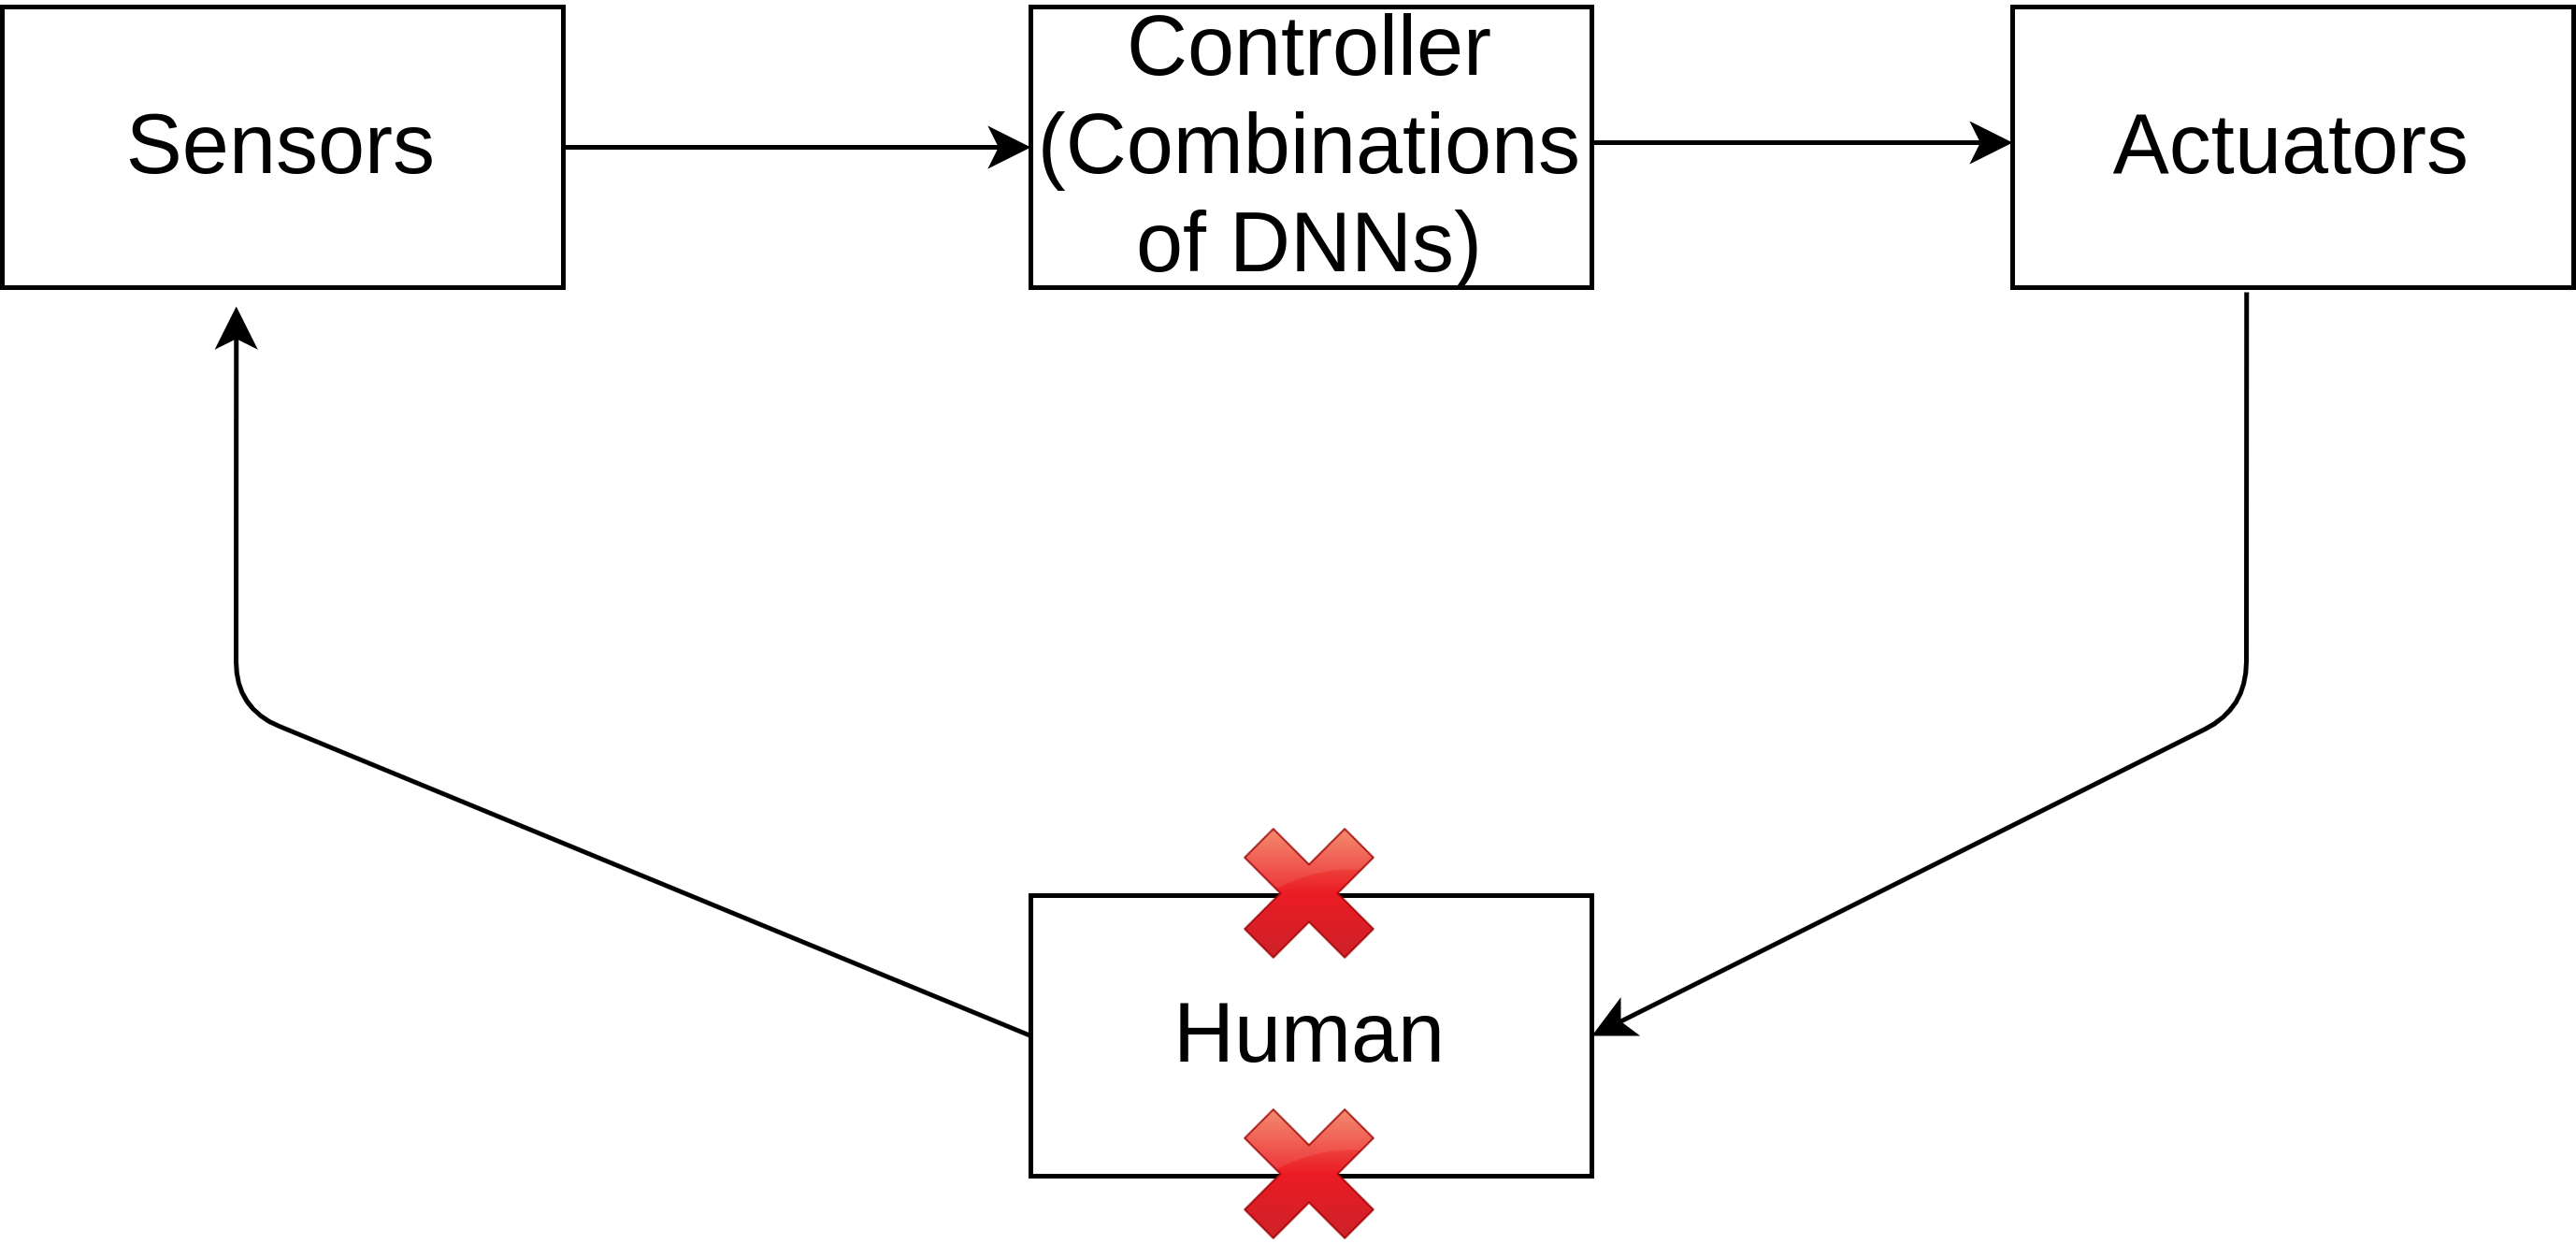
\includegraphics[width=0.7\linewidth]{Images/Systemsdescription}
	\caption{Architecture of a CPS}
	\label{fig:systemsdescription}
\end{figure}

\begin{figure}
	\centering
	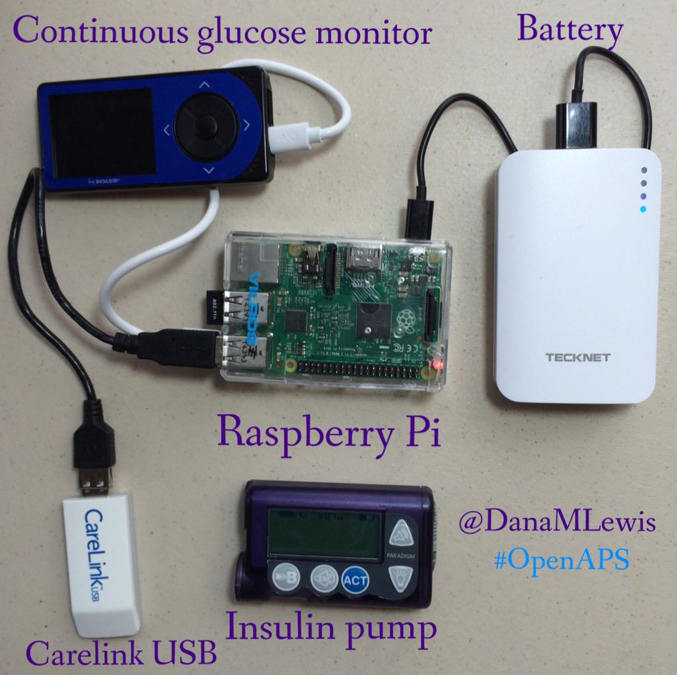
\includegraphics[width=0.7\linewidth]{Images/APSrig}
	\caption{Artifical Pancreas System components \\
		Source: www.openAPS.org}
	\label{fig:apsrig}
\end{figure}



\begin{figure}
	\centering
	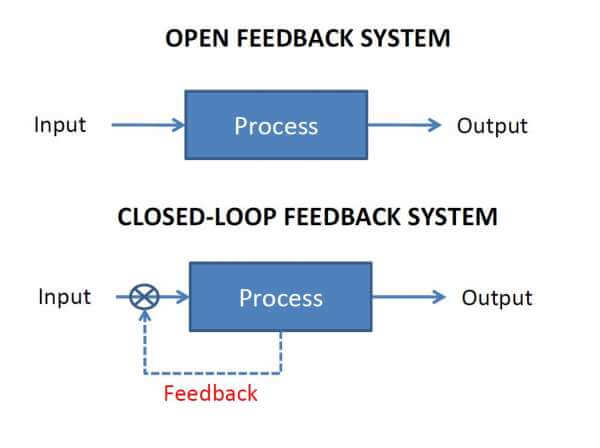
\includegraphics[width=0.7\linewidth]{Images/closedvsopen}
	\caption{General structure of a open and closed-loop systems 
		Source:https://instrumentationtools.com/open-loop-and-closed-loop-animation/ }
	\label{fig:closedvsopen}
\end{figure}


\section{Cyber-Physical Systems}
\ac{CPS} are systems that perform computations in the cyber part to reflect changes in the physical  part.   
As shown in Figure ~\ref{fig:systemsdescription} the sensors and actuators are the physical parts of the system. 
The sensors gather the data from the physical environment and send it to the computational unit. 
The decision is taken at the computational unit which is also the cyber part of the \ac{CPS} called the controller.
The decision is sent to the actuator which then physically performs the action.
The physical and virtual contexts can either be humans in the loop or some automated mechanism.

In an \ac{APS} shown in Figure ~\ref{fig:apsrig}, the sensor is the \ac{CGM} that is attached to the back of a patient to report the blood glucose levels.  
\ac{RPi} is the computational part of the \ac{APS}, and the insulin pump is the actuator. 

There are two types of CPS based on the decision making process: open feedback and closed-loop feedback.
In open feedback systems, there is human intervention during the decision making process. 
As shown in Figure ~\ref{fig:closedvsopen} (top diagram), the human is a part of the loop where he/she keeps track of the decisions being taken by the controller. 
In closed-loop systems, there are no human interventions 
as shown in Figure ~\ref{fig:closedvsopen} (below diagram). 
In the latter case, understanding different types of security attacks becomes a necessity because the automation means that once the attacker has found a way to tamper the automation mechanism, they can fool the system. 
In the case of stealthy (or subtle) attacks as described in Chapter 3, 
the closed loop systems are more vulnerable because existing error-detection mechanisms can be reverse engineered and can be used to attack the systems. 

\section{Conventional Controllers for CPS}

A conventional controller takes in the sensors readings and processes the input based on the different sets of differential equations for the controller. 
For instance, a quadcopter contains multiple flight modes in its controller based on the weather conditions such as windy or normal day. 
These modes are important because during windy weather, the decision making model for stable quadcopter flights will be different from a normal weather flight \cite{inbook}. 

Based on the inputs or data collected from the sensors, the appropriate  mode is selected and the decision is calculated. 
Every mode consists of a different set of equations because every mode represents a different scenario.
Figure ~\ref{fig:controltheory} shows a position control system of a quadcopter \cite{inbook}. The input values use the derived version of the equations that are used in decision making. 

\begin{figure}
	\centering
	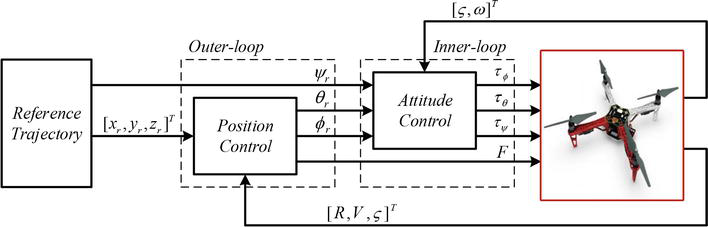
\includegraphics[width=0.7\linewidth]{Images/controltheory}
	\caption{The block diagram of the position control system of the quadcopter.
	}
	\label{fig:controltheory} 
\end{figure}


%How are they modeled
These modes are modeled using classical control theory that is represented as a set of equations designed by domain experts.
For instance, the model for a medical system such as \ac{APS} can be designed only if the specifications are known for the medical system. 
A part of the specifications such as the important parameters (insulin, blood glucose etc. in APS) and their threshold values are be provided by domain (in this case medical) experts. 
Another important aspect for designing control systems is modeling the precise relations between the parameters. 
This is possible in systems such as APS because it is a simpler system as compared to self-driving cars. 
However, designing the precise mathematical relations for systems such as self-driving cars can be tedious \cite{article23}, as we elaborate below.

The move towards DNNs over control theory models for modeling \ac{CPS} behaviour can be justified by the following observations:
\begin{enumerate}
	\item CPS behaviour is controlled using a lot of input data from the many sensors a system might have. The self-learning nature of DNNs lends itself well to model behaviour that is driven by the sensor input. This is easier than formulating the control theoretic differential equations, which need domain and mathematical expertise \cite{Aamir_2013}.
	
	
	To look at a more concrete example, let us turn to a medical system such as \ac{APS}, which uses conventional control theory to build models. 
	Forming the model requires the programmer to be aware of not only the intended system behaviour, but also the mathematical rigor needed to get the desired result. 
	DNNs, on the other hand, can automatically build models with data.
	Training DNNs is implicitly dependent on the quality of available training data, and it is a known problem in the field \cite{jabbar2015methods}. It does not, however, require the system designers to model precise control equations like in control theory.
	\item  There are limitations on the behaviors that can be modeled using the standard control-theoretic approaches. They do not, for instance, work well for building dynamic models \cite{article23}. Building such dynamic models is important in many systems such as in autonomous vehicles, which are essentially composed of multiple interacting control systems. Conventional control systems are not designed to work in an interactive, plug-and-play manner with other control systems because they are built to model only one behaviour. DNNs, by their very nature,  provide this dynamic capability \cite{article23}. 
	Due to the data driven modeling using DNNs, it is relatively easier to build models for autonomous vehicles that have multiple models interacting within them.
	For instance, they contain separate models for image recognition and lane detection that continuously interact with each other to decide the next best course of action.
	
	\item Sarabakha et al. \cite{sarabakha2019online} show that using \ac{DNN} based controller for a quadcopter leads to better decision making in un specified cases as compared to control theory models.
	This is due to the learning nature of \ac{DNN}s in contrast to the fixed nature of conventional control theory. 
	Hence, in cases when the trajectories or situations are not precisely modeled, the \ac{DNN} comes closer to taking good decisions.
\end{enumerate}




\section{DNN Based Controller}
\label{apsdnn}


%A \ac{NN} is an algorithm that is modeled after the human brain.
A \ac{NN} consists of input, output and hidden layers. 
The layers are built of nodes. Every computation occurs within in a node of a network.
In the base case, there is a single neuron that takes all the inputs to produce an output as shown in Figure 2.5. 
All inputs to the node in Figure 2.5 are summed and are passed through an activation function. 
The activation function introduces non-linearity in the network. 
The node determines upto what extent the signal must be progressed to calculate the final output. 
The final output depends on the network and can be in binary form or have a value associated with it. 


A \ac{DNN} consists of multiple hidden layers as apposed to our base case  as shown in Figure 2.7.
This is an example of a feed-forward \ac{DNN} which is the simplest type of artificial neural network devised \cite{feedforward}.
In this network, the information flows only forward from inputs, through layers, to outputs \cite{Zell}. 

The classical controller model is being replaced by such DNN based controllers for CPS as shown in  Figure 2.6.
The \ac{DNN} for \ac*{CPS} is trained using the data gathered from conventional control equations. 
One example is the DNN based controller designed by Dutta et al. \cite{Dutta_Others__2018__Robust}. 
Dutta et al. model robust DNN using available patient data to predict the output for an insulin pump.
Their controller design is for providing a data-driven approach for an artificial pancreas system (APS) which is also our first system for evaluation. 

We evaluate two other systems called \ac{CA} systems for unmanned vehicles \cite{7778055} called \ac{HCAS} and \ac{ACAS-Xu}: both \ac{CA} are bigger in size (number of nodes and layers) and have a complex architecture in terms of design as compared to \ac{APS}.


%Normalization layers in DNN
\ac{DNN}s also consist of a feature called normalization in their layers. 
This feature exist mostly in \ac{DNN}s as compared to other \ac{ML} models such as decision trees etc. since \ac{DNN}s involves less feature engineering as compared to other models. 
Feature engineering is the automatic means to extract features automatically from raw data. 
Normalization is a common feature engineering method where all the inputs are brought to standard scale since different set of inputs can be in different ranges. 
This is important in \ac{DNN}s for reasons explained by  LeCun et al.  \cite{10.5555/645754.668382}.
%The first reason is trivial as computations on a bounded range of numbers prevent some numerical inaccuracies and limit the computational power required. The second reason is that some machine learning algorithms can handle that data better when it is normalized. There are several approaches to normalization of the data.
Our other two evaluation systems are air craft  control management systems \cite{10.1007/978-3-319-63387-9_5} that consist of a normalization layer, 
which we have to consider in our system modeling. 
\subsection{Understanding DNN complexity}
\label{dnncomplexity}
To understand the complexity of \ac{DNN}s we use two criteria
\begin{enumerate}
	\item Size: The size depends on two aspects, the number of layers in a \ac{DNN} and the number of nodes in each layer. 
    The increase in the hidden layers corresponds to more connections and opacity between the inputs and the outputs. 
    The increase in the number of nodes per layer corresponds to more connections between each layer which ultimately increases the opacity of the input and output mapping. 
	\item Architecture: The architecture consists of the the design of the network. 
	For a fully-connected network, all nodes are connected to every other node in the network and it contains ReLU or some other activation function to introduce non-linearity.
	Other networks also consist of layers that perform max/average pooling operations. 
	
\end{enumerate}
When we refer to \ac{DNN} complexity in the later sections we are referring to the difference in size and architecture.


\begin{figure}
	\centering
	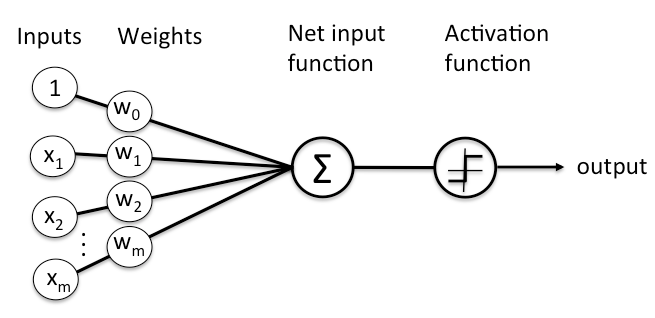
\includegraphics[width=0.7\linewidth]{Images/perceptron_node}
	\caption{Perceptron node  \\ Source: https://pathmind.com/wiki/neural-network}
	\label{fig:perceptronnode}
\end{figure}

\begin{figure}
	\centering
	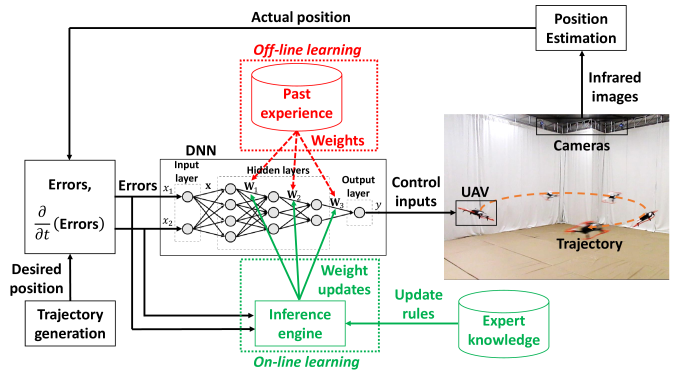
\includegraphics[width=0.7\linewidth]{Images/DNNcontroller}
	\caption{Illustration of how DNN controllers are replacing conventional controllers. The DNN is trained offline using input-output data obtained from different trajectories from a conventional controller. The DNN is shown to perform better than a conventional controller during real-time analysis for decision making.}
	\label{fig:dnncontroller}
\end{figure}

\begin{figure}
	\centering
	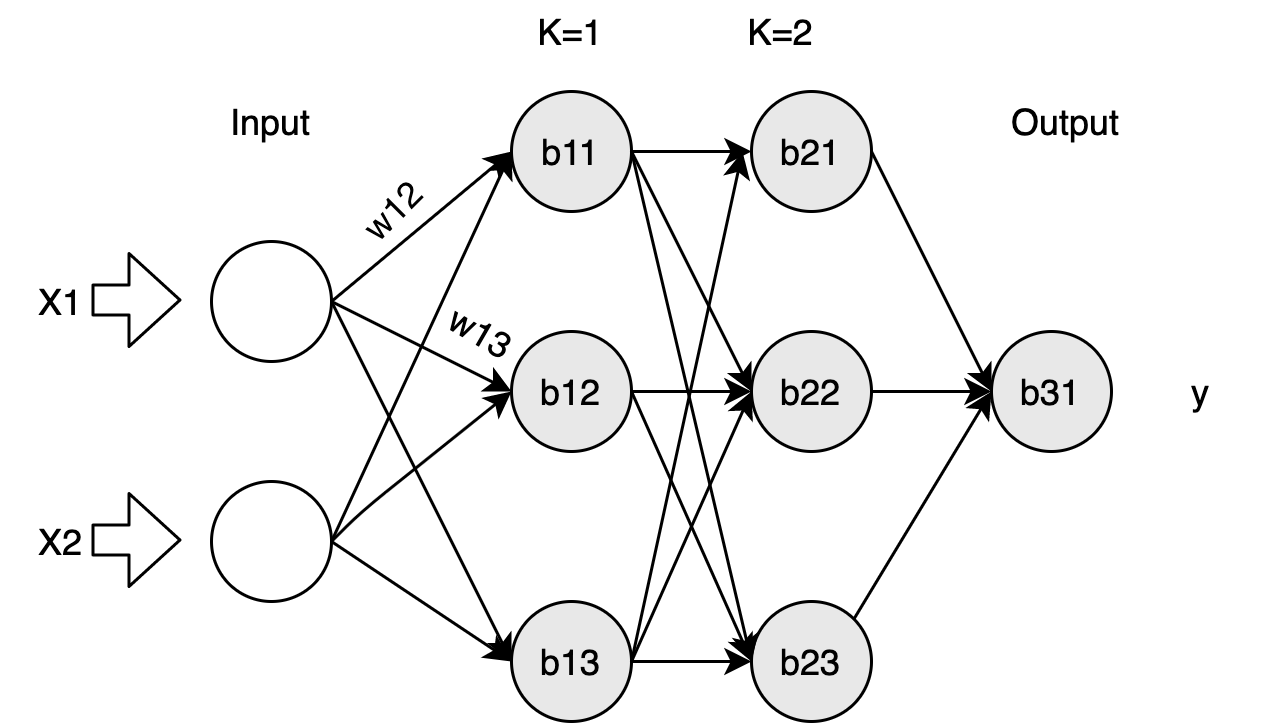
\includegraphics[width=0.7\linewidth]{Images/DNNstructure}
	\caption[DNN structure]{DNN controller structure with two hidden layers K=1,2, two inputs x1 and x2 and one output y. This is an example of a fully connected network.}
	\label{fig:dnn-controller}
\end{figure}

\section{Modeling Mixed-Integer Linear Programming Problems}

We present a general structure that is required for building a \ac{LP} \ac{MILP} models.
The reason we are introducing the notion of \ac{MILP} is because we use the modeling techniques underlying \ac{MILP} to model \ac{DNN}s and systematically reason about them. 


\ac{LP} consists of the following components. 

\begin{enumerate}
	\item A \ac{LP} contains a set of decision variables, which are the unknown quantities or decisions that are to be optimized. 
	\item The function that assess the quality of the solution is called an objective function or the cost function.
	\item \ac{LP}'s goal is to minimize or maximize the value of an objective function. 
	The decisions that are to be made depends on the requirements, and restrictions of the  system modeled as \ac{LP}.
	\item A solution that satisfies all constraints is called a feasible solution. 
	Feasible solutions that achieve the the best cost function value, depending on weather one is minimizing or maximizing are called as optimal solutions. 
\end{enumerate}


The general form of a \ac{LP} looks as shown in Equations 2.1. 
Values of $c$ denote the objective coefficients, and are often associated with their corresponding decisions minimization problems. 
$x_i$ denotes the set of our decision variables.
$b_i$ denotes the requirements of the constraints. 
A very important point here is that nonlinear terms are not allowed in the model. 
Hence, something as simple as multiplication of two decision variables is prohibited in the model representation. 
\begin{equation}
\begin{aligned}
& \underset{x}{\text{min/max}}
& & c^T x \\
& \text{subject to} & &  Ax \leq b_i \\
& & &  \sum_{i=1}^{n} x_i =1 \\
& & &  x_j, \; \forall j \in N. \\
\end{aligned}
\end{equation}

A \ac{MILP} is a \ac{LP} with a restriction that some of the variables in the model must be integer-valued. 
We define a \ac{DNN} as a \ac{MILP} model due to the complex structure of a \ac{DNN} which we will elaborate more in Chapter 5. 



\section{Problem Statement}

Given a trained DNN with fixed parameters our goal is to understand if the well-known \ac*{FDIA} in classical control theory are also valid in the DNN based CPS.
\begin{problem}
	How can we identify the critical inputs in a DNN?
\end{problem}

\begin{problem}
	What is the smallest perturbation to the critical input(s) that can produce \ac{RFDIA}?
\end{problem}




